\documentclass[12pt]{report}
\usepackage[T1]{fontenc}
\usepackage[utf8]{inputenc}
\usepackage{lmodern} %textcomp for usage of euro currency symbol
\usepackage{listings}
\usepackage[margin=1in]{geometry}
\usepackage{csquotes}
\usepackage[english]{babel}
\usepackage{color}
\usepackage{xcolor} %for more colours to use in hyperref
\usepackage{amsmath}
\usepackage{amssymb}
\usepackage{caption}
\usepackage{subcaption}
\usepackage{mathpazo}


\usepackage{makecell} %for resizing hline
\usepackage{float}
\usepackage{graphicx} %for pictures
\graphicspath{ {figures/} }
\usepackage[
    backend=biber,
    style=numeric,
    sorting=none
    ]{biblatex}
\addbibresource{ref.bib}

\usepackage{hyperref}
\hypersetup{
    colorlinks=true, %set true if you want colored links
    linkcolor={red!50!black},
    citecolor={blue!50!black},
    urlcolor={blue!80!black}
    }
    
\usepackage{listings}
\usepackage{color}
\usepackage{mathtools}


\usepackage{graphicx}
\usepackage{caption}
\usepackage{subcaption}

\definecolor{mygreen}{rgb}{0,0.6,0}
\definecolor{mygray}{rgb}{0.5,0.5,0.5}
\definecolor{mymauve}{rgb}{0.58,0,0.82}

\lstset{ %
  backgroundcolor=\color{white},   % choose the background color; you must add \usepackage{color} or \usepackage{xcolor}; should come as last argument
  basicstyle=\footnotesize,        % the size of the fonts that are used for the code
  breakatwhitespace=false,         % sets if automatic breaks should only happen at whitespace
  breaklines=true,                 % sets automatic line breaking
  captionpos=b,                    % sets the caption-position to bottom
  commentstyle=\color{mygreen},    % comment style
  deletekeywords={...},            % if you want to delete keywords from the given language
  escapeinside={\%*}{*)},          % if you want to add LaTeX within your code
  extendedchars=true,              % lets you use non-ASCII characters; for 8-bits encodings only, does not work with UTF-8
  frame=single,	                   % adds a frame around the code
  keepspaces=true,                 % keeps spaces in text, useful for keeping indentation of code (possibly needs columns=flexible)
  keywordstyle=\color{blue},       % keyword style
  language=Octave,                 % the language of the code
  morekeywords={*,...},           % if you want to add more keywords to the set
  numbers=left,                    % where to put the line-numbers; possible values are (none, left, right)
  numbersep=5pt,                   % how far the line-numbers are from the code
  numberstyle=\tiny\color{mygray}, % the style that is used for the line-numbers
  rulecolor=\color{black},         % if not set, the frame-color may be changed on line-breaks within not-black text (e.g. comments (green here))
  showspaces=false,                % show spaces everywhere adding particular underscores; it overrides 'showstringspaces'
  showstringspaces=false,          % underline spaces within strings only
  showtabs=false,                  % show tabs within strings adding particular underscores
  stepnumber=2,                    % the step between two line-numbers. If it's 1, each line will be numbered
  stringstyle=\color{mymauve},     % string literal style
  tabsize=2,	                   % sets default tabsize to 2 spaces
  title=\lstname                   % show the filename of files included with \lstinputlisting; also try caption instead of title
}

\usepackage{algorithm}
\usepackage[noend]{algpseudocode}
\makeatletter
\def\BState{\State\hskip-\ALG@thistlm}
\makeatother

\newcommand*\samethanks[1][\value{footnote}]{\footnotemark[#1]}

\title{\Large{\textbf{FE Project}}\\\Large{IEORE 4706 Foundations for Financial Engineering}}

\author{
    Ahmad Shayaan\thanks{All authors contributed equally to this work.} \\as5948
    } 

\date{
\{\href{mailto:ahmad.shayaan@columbia.edu}{\texttt{\small{ahmad.shayaan@columbia.edu}}}\}\texttt{\small{@columbia.edu}}\\
    Columbia University\\
    \today}



\usepackage[utf8]{inputenc}

% Default fixed font does not support bold face
\DeclareFixedFont{\ttb}{T1}{txtt}{bx}{n}{12} % for bold
\DeclareFixedFont{\ttm}{T1}{txtt}{m}{n}{12}  % for normal

% Custom colors
\usepackage{color}
\definecolor{deepblue}{rgb}{0,0,0.5}
\definecolor{deepred}{rgb}{0.6,0,0}
\definecolor{deepgreen}{rgb}{0,0.5,0}

\usepackage{listings}

% Python style for highlighting
\newcommand\pythonstyle{\lstset{
		language=Python,
		basicstyle=\ttm,
		otherkeywords={self},             % Add keywords here
		keywordstyle=\ttb\color{deepblue},
		emph={MyClass,__init__},          % Custom highlighting
		emphstyle=\ttb\color{deepred},    % Custom highlighting style
		stringstyle=\color{deepgreen},
		frame=tb,                         % Any extra options here
		showstringspaces=false            % 
	}}
	
	
	% Python environment
	\lstnewenvironment{python}[1][]
	{
		\pythonstyle
		\lstset{#1}
	}
	{}
	
	% Python for external files
	\newcommand\pythonexternal[2][]{{
			\pythonstyle
			\lstinputlisting[#1]{#2}}}
	
	% Python for inline
	\newcommand\pythoninline[1]{{\pythonstyle\lstinline!#1!}}
	
\newcommand{\defeq}{\vcentcolon=}

\begin{document}

\maketitle
\tableofcontents

\pagebreak

\chapter*{Perpetual American Options}
\addcontentsline{toc}{chapter}{\protect\numberline{Perpetual American Options}}

\section*{Exercise region}
\addcontentsline{toc}{section}{\protect\numberline{Exercise Region}}
For a put option the pay-off is only positive if the value of the underlying security is less than the strike price. Thus if $x^*$ is the optimal price at which we exercise the option then, necessarily for a positive payoff $x^*$ has to be less than $K$. This means that the range of values for $x^*$ is $(0,K]$, 0 is not included in the range because if the value of the underlying security hit 0 it cannot be traded in the market. We also know that the yield of a put option increases with a decrease in the value of the underlying security. Thus if it is optimal to exercise the option at $x^*$ it will always be optimal to exercise the option for all the prices of the security that are below $x*$. Thus the range of the price of the security ($S$) is $(0,x^*]$. Again 0 is not included because if the value of the security becomes zero it cannot be traded on the market.

\section*{Solution of the differential equation}
\addcontentsline{toc}{section}{\protect\numberline{Solution of the differential equation}}
If $x > x^*$ this will mean that the exercise is not optimal, and the payoff of the option is less than the value i.e. $v(x) - h(x) > $. Thus from the Hamilton-Jacobi-Bellman equation $v$ must satisfy the following differential equation.

\begin{equation*}
	\begin{aligned}
		rv(x) -\mu xv'(x) - \frac{1}{2} \sigma^2 x^2 v''(x) &= 0 \\
		x^2v''(x) + \frac{2\mu x}{\sigma^2}v'(x) - \frac{2r}{\sigma^2} v(x) = 0
	\end{aligned}
\end{equation*}

Let the solution to the above general equation be $v(x) = x^\lambda$. Then $v'(x) = \lambda x^{(\lambda-1)}$ and $v''(x) = \lambda (\lambda-1) x^{(\lambda-2)}$. Thus the above equation becomes.

\begin{equation*}
	\begin{aligned}
		\lambda (\lambda-1) x^\lambda + \frac{2\mu =x}{\sigma^2} \lambda x^\lambda - \frac{2r}{\sigma^2} x^\lambda &= 0\\
		\lambda (\lambda -1) + \frac{2\mu x}{\sigma^2} \lambda - \frac{2r}{\sigma^2} & =0 \\
		\sigma^2 \lambda^2 + {(2\mu - \sigma^2)}\lambda - {2r} &=0 \\
		\lambda &= \frac{-(2\mu - \sigma^2) \pm \sqrt{(2\mu - \sigma^2)^2 + 8\sigma r} }{2\sigma^2} 	
	\end{aligned}
\end{equation*}

Let m and n be the solution to the equation. Then

\begin{equation*}
	\begin{aligned}
		m & = \frac{-(2\mu - \sigma^2) - \sqrt{(2\mu - \sigma^2)^2 + 8r\sigma} }{2\sigma^2} \\
		n &= \frac{-(2\mu - \sigma^2) + \sqrt{(2\mu - \sigma^2)^2 + 8r\sigma} }{2\sigma^2}  
	\end{aligned}
\end{equation*}

Where $m\leq0$ and since $8r\sigma^2 >0$ , $n\geq0$. Thus $v(x)$ is given by.

\begin{equation*}
\begin{aligned}
	v(x) &= Ax^m + Bx^n\\
	m & = \frac{-(2\mu - \sigma^2) - \sqrt{(2\mu - \sigma^2)^2 + 8r\sigma} }{2\sigma^2} \\
	n &= \frac{-(2\mu - \sigma^2) + \sqrt{(2\mu - \sigma^2)^2 + 8r\sigma} }{2\sigma^2}  
\end{aligned}	
\end{equation*}

\section*{Boundedness of value of option}
\addcontentsline{toc}{section}{\protect\numberline{Boundedness of value of option}}

Let us assume that $v(x)$ is not bounded then there definitely exists a $x$ such that $v(x) > K$. We sell the put whose value is K and put the money in the bank at time t. Then there are two cases.

Case 1. The put is exercised at time $\tau$ . If this happens then we take the money out of the bank to fund the exercise of the put. Thus in this case the profit is given by.

\begin{equation*}
	-(K-x^*)^+  + K/d(0,\tau) > 0
\end{equation*}


Case 2. The put is not exercised till maturity $T$. Then in that case the payoff is.

\begin{equation*}
	-(K-x^*)^+  + K/d(0,\tau) > 0
\end{equation*}

We have an arbitrage opportunity in both the cases. Since there are no arbitrage opportunities in the market thus are assumption that  $v(x) > K$ is wrong. Thus we can conclude that $v(x) \leq K$ and bounded.

We have proved that $v(x) \l K$ which implies that $Ax^m + B \leq K \ \forall x$. 

\begin{equation*}
	\begin{aligned}
		lim_{x\rightarrow \infty} v(x) & \leq K\\
		\implies lim_{x\rightarrow \infty} Ax^m + Bx^n & \leq K\\ 
		\implies lim_{x\rightarrow \infty} Ax^ m + lim_{x\rightarrow \infty} Bx^m & \leq K \hspace{2cm} \text{$\because m < 0$} \\
		\implies lim_{x\rightarrow \infty} Bx^n \leq K \\
		\implies B &= 0 \hspace{2cm} \text{$\because n >1$}
	\end{aligned}
\end{equation*}

\section*{Optimal exercise}
\addcontentsline{toc}{section}{\protect\numberline{Optimal Exercise}}
From the second section we can conclude that any $x \leq x^*$  we have $v(x) = h(x) \implies  Ax^m = (K-x)$. Since value of a option are continuous we can differentiate wrt x. 

\begin{equation*}
	\begin{aligned}
		\frac{dv(x)}{x}|_{x=x^*} &=  \frac{dh(x)}{dx}|_{x=x^*} \\
		\implies \frac{d(AX^m)}{dx}|_{x=x^*} &= \frac{d(K-x)}{dx}|_{x=x^*} \\
		\implies mAx^{*(m-1)} &= -1 \\
		\implies mAx^{*m} &= -x^* \\
		\implies m (K-x^*) &= -x^* \\
		\implies x^* &= \frac{mK}{(m-1)}
	\end{aligned}	
\end{equation*}

Substituting the value of $x^*$ in the equation $  Ax^{*m} = (K-x^*)$.

\begin{equation*}
	\begin{aligned}
	A & = \frac{(K-x^*)}{x^{*m}} \\
	A &=  \frac{(K - \frac{mK}{(K-1)})}{\Big[\frac{mK}{(K-1)}\Big]^m}
	\end{aligned}
\end{equation*} 

From the above results we can conclude that it is optimal to exercise the option when $x \leq \frac{mK}{(m-1)} \leq K$.
\linebreak
\linebreak
From the previous section we know that $m$ is given by $m = \frac{-(2\mu - \sigma^2) - \sqrt{(2\mu - \sigma^2)^2 + 8\sigma r} }{2\sigma^2}$. We now need to find the limit when $r\rightarrow 0$. 
\begin{equation*}
	\begin{aligned}
		&lim_{r \rightarrow 0} m \\
		&= lim_{r \rightarrow 0} m = \frac{-(2\mu - \sigma^2) - \sqrt{(2\mu - \sigma^2)^2 + 8\sigma r} }{2\sigma^2}\\
		&= 0 
	\end{aligned}
\end{equation*}

We  now need to find the limit of $x^*$ as r tends to zero.

\begin{equation*}
	\begin{aligned}
		&lim_{r \rightarrow 0} x^*\\
		&= lim_{r \rightarrow 0} \frac{mK}{m-1} \\
		&= lim_{m \rightarrow 0} \frac{mK}{m-1} \\
		&= 0
	\end{aligned}
\end{equation*}

Now we need to find A as r tends to zero.

\begin{equation*}
\begin{aligned}
	&lim_{r \rightarrow 0} A\\
	&= lim_{m \rightarrow 0}  A \\
	&= lim_{m \rightarrow 0} \frac{-K}{m-1} \Big[\frac{m-1}{mK} \Big]^m\\
	\implies lim_{m \rightarrow 0} \log A &= lim_{m \rightarrow 0} \log\frac{-K}{m-1} + lim_{m \rightarrow 0} m \log \frac{m-1}{mk} \\
	\implies lim_{m \rightarrow 0} \log A &= \log K + lim_{m \rightarrow 0} \frac{\log \frac{m-1}{mk}}{\frac{1}{m}} \\ 
	\implies lim_{m \rightarrow 0} \log A &= \log K	\\
	\implies lim_{m \rightarrow 0} A &= K\\
	\implies lim_{r \rightarrow 0} A &= K
\end{aligned}
\end{equation*}

\chapter*{Pricing using CRR model}
\addcontentsline{toc}{chapter}{\protect\numberline{Pricing using CRR model}}

In this question we had use the Cox-Ross-Rubinstein model valuation for valuation of options. The CRR model is a discrete time pricing model in which the evolution of the risky asset is given by.

\begin{equation*}
	S_{t_{i+1}} = S_{t_{i}}U^{i}
\end{equation*}	

Where $U^i$ is the up state (u) or the down state (d).

\begin{equation*}
	u \defeq e^{\sigma \sqrt{\frac{T}{n}} }
\end{equation*}
\begin{equation*}
	d \defeq e^{-\sigma \sqrt{\frac{T}{n}} }
\end{equation*}

Where $\sigma$ is the volatility of the underlying security, T is the time at which the security matures and n is the depth of the tree. 

\section*{Building the tree}
\addcontentsline{toc}{section}{\protect\numberline{Building the tree}}
We had to create the binomial price tree for the risky asset. The tree is generated by using a matrix of size $(n+1) \times (n+1)$, where n is the depth of the tree. The matrix is filled by working forward from the date of valuation to the date of maturity of the underlying security. At each step, it is assumed that the underlying security can move up by a factor of u or down by a factor of d. The code used to generate the price tree of the underlying security is shown below.
\
\begin{tiny}
\begin{python}
def buildTree(self):
 for i in range(self.n+1):
   for j in range(i+1):
     self.tree_security[i][j] = self.security_price * math.pow(self.u,j) * math.pow(self.d,i-j)
	\end{python}	
\end{tiny}

\section*{Pricing European and American options}
\addcontentsline{toc}{section}{\protect\numberline{Pricing European and American options}}
We had to come up with a recursive formula for valuation of European and American options at every node of the tree. At the terminals nodes i.e. at the maturity of the option, the option value is simply the exercise value. 

\begin{equation*}
	\begin{aligned}
		max[(S_T - K),0] \ \ \  \text{American and European call option} \\
		max[(K - S_T),0] \ \ \  \text{American and European put option}
	\end{aligned}
\end{equation*}

Once the valuation is computed at the terminal nodes, the valuation at every other node can be computed as the discounted expected value of the pay off under the risk neutral measure. In CRR model the risk-neutral measure is given by.

\begin{equation*}
	q \defeq \mathbb{Q}[U^i = u] = \frac{e^{R \frac{T}{n}} - d}{ u - d}
\end{equation*}

And the value of the option at each node for a European options are given by. 

\begin{equation*}
	S_{t_i} = e^{-rT/n} \Big[ qS_{t_{i+1}}\{U^i=u\} + (1-q)S_{t_{i+1}}\{U^i=D\}\Big]
\end{equation*}

S in the above recursion represents the price of the option. With America  options we have the choice of exercising early and the value at every node is given by.

\begin{equation*}
	\begin{aligned}
		S_{t_i} &= max\Big[(SP_{t_i} - K), e^{-rT/n} \big[ qS_{t_{i+1}}\{U^i=u\} + (1-q)S_{t_{i+1}}\{U^i=D\}\big] \Big]  \ \text{American Call}\\
		S_{t_i} &= max\Big[(K - SP_{t_i}), e^{-rT/n} \big[ qS_{t_{i+1}}\{U^i=u\} + (1-q)S_{t_{i+1}}\{U^i=D\}\big] \Big] \  \text{American Put}
	\end{aligned}
\end{equation*}

SP in the above recursion is the price of the underlying security which we get from the tree that was computed early. The code that was used to compute the valuation of the American and European options is shown below.
\begin{tiny}
	\begin{python}

	def computePrice(self):
	 for i in range(self.n-1,-1,-1):
	  for j in range(i+1):
		if self.type == 'European Call':
		 self.tree_option[i][j] = math.exp(-1*self.rate*self.deltaT)
								          *((1-self.p) * self.tree_option[i+1][j] 
								          + (self.p)*self.tree_option[i+1][j+1])
		
		elif self.type == 'European Put':
		 self.tree_option[i][j] = math.exp(-1*self.rate*self.deltaT)
		                      *((1-self.p) * self.tree_option[i+1][j] 
		                       + (self.p)*self.tree_option[i+1][j+1])
		
		elif self.type == 'American Call':
		 self.tree_option[i][j] = max(self.tree_security[i][j]-
		                          self.strike_price,
		                         math.exp(-1*self.rate*self.deltaT)
		                        *((1-self.p)*self.tree_option[i+1][j] 
		                     + (self.p)*self.tree_option[i+1][j+1]))
		
		elif self.type == 'American Put':
		 self.tree_option[i][j] = max(self.strike_price
		                       -self.tree_security[i][j],
		                       math.exp(-1*self.rate*self.deltaT)
		                       *((1-self.p)*self.tree_option[i+1][j]
		                       +(self.p)*self.tree_option[i+1][j+1]))
		 #Finding the exercise frontier
		 if self.tree_option[i][j] == (self.strike_price-self.tree_security[i][j]):
          self.EPA[i][j] = 1
\end{python}
\end{tiny}

We compared the values of American call and put when the interest rate are taken to zero. The value of the American call option decreased when the interest rate is brought down to zero. Whereas the value of the American option increased when we brought the interest down to zero. 

From the American call put party we know that.
\begin{equation*}
	\begin{aligned}
		S_t - K \leq C^A_t(T,K,S) - P^A_t(T,K,S)  \leq S_t - Kd(t,T)
	\end{aligned}
\end{equation*}

When the interest go down to zero we get that.

\begin{equation*}
\begin{aligned}
	C^A_t(T,K,S) - P^A_t(T,K,S) = S_t - K
\end{aligned}
\end{equation*}

In the implementation of your model we have set the initial value of the security and strike to be the same, thus at time $t=0$ we get the values of the call and put option to be the same.

\begin{equation*}
\begin{aligned}
C^A_0(T,K,S) = P^A_0(T,K,S)
\end{aligned}
\end{equation*}

In the cases where the initial value of the security and strike are not same. The value of call and put options are related as follows.

\begin{equation*}
	\begin{aligned}
		C^A_0(T,K,S) = P^A_0(T,K,S) + S_0 - K
	\end{aligned}
\end{equation*}

From the above relation we can conclude that if the strike is selected such that it is greater than the initial value of the security then the value of American call will be less than an American put when interest rates are zero and vice-versa. 



\section*{Exercise frontier of an American put}
\addcontentsline{toc}{section}{\protect\numberline{Exercise Frontier of an American Put}}
Once the valuation of the American put option had been done we had to find the optimal exercise frontier of the American Put and study its relation to the interest rate and the depth of the tree in CRR model. We plotted the exercise frontier for different values of depth and interest rate.
\begin{small}
\begin{figure}[H]
	\begin{subfigure}{.5\textwidth}
		\centering
		% include first image
		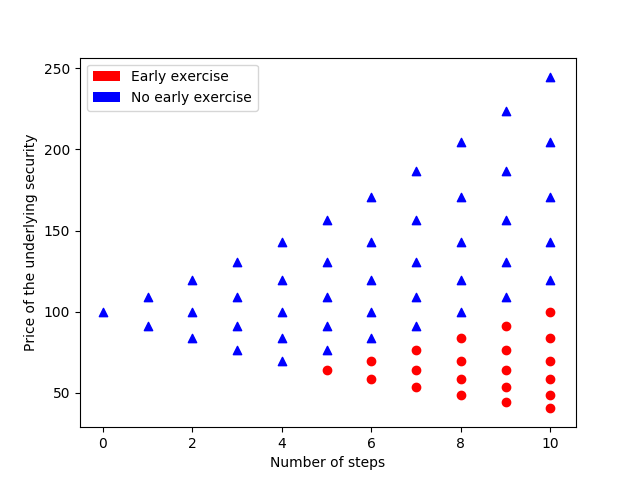
\includegraphics[width=.8\linewidth]{plots/n_10_r_001.png}  
		\caption{0.1\% interest}
		\label{fig1:sub-first}
	\end{subfigure}
	\begin{subfigure}{.5\textwidth}
		\centering
		% include second image
		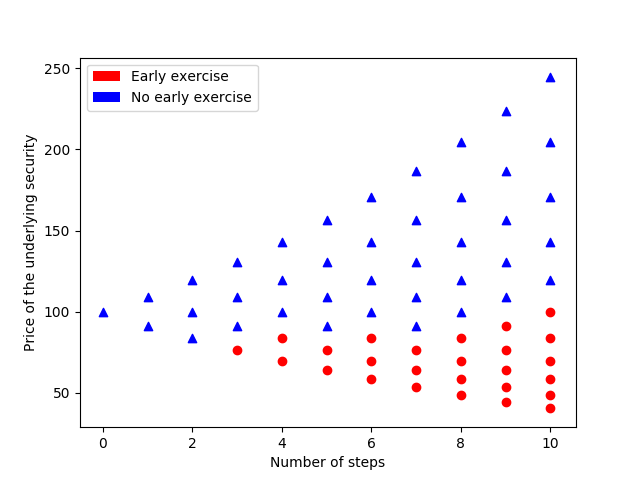
\includegraphics[width=.8\linewidth]{plots/n_10_r_005.png}  
		\caption{5\% interest}
		\label{fig1:sub-second}
	\end{subfigure}
	
	
	\begin{subfigure}{.5\textwidth}
		\centering
		% include third image
		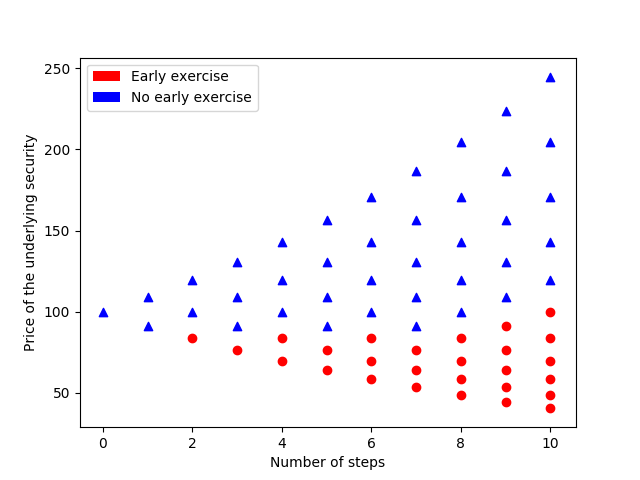
\includegraphics[width=.8\linewidth]{plots/n_10_r_01.png}  
		\caption{10\% interest}
		\label{fig1:sub-third}
	\end{subfigure}
	\begin{subfigure}{.5\textwidth}
		\centering
		% include fourth image
		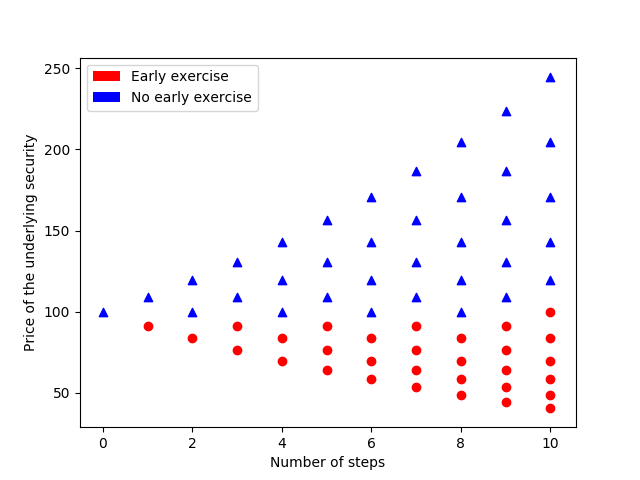
\includegraphics[width=.8\linewidth]{plots/n_10_r_015.png}  
		\caption{15\% interest}
		\label{fig1:sub-fourth}
	\end{subfigure}
	\caption{Interest rate variation in a tree of depth 10}
	\label{fig:fig1}
\end{figure}
\end{small}

It can be observed from the figures that for the same depth the exercise frontier moves up in the tree i.e. when we increase the interest rate we can optimally exercise an American option earlier.

\begin{small}
	\begin{figure}[H]
		\begin{subfigure}{.5\textwidth}
			\centering
			% include first image
			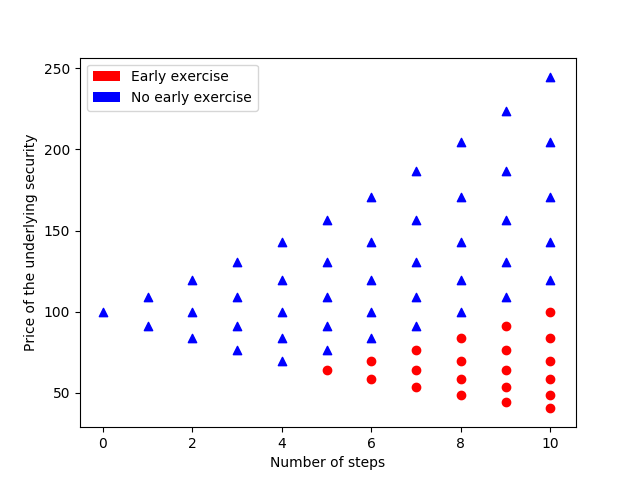
\includegraphics[width=.8\linewidth]{plots/n_10_r_001.png}  
			\caption{Tree with depth 10}
			\label{fig2:sub-first}
		\end{subfigure}
		\begin{subfigure}{.5\textwidth}
			\centering
			% include second image
			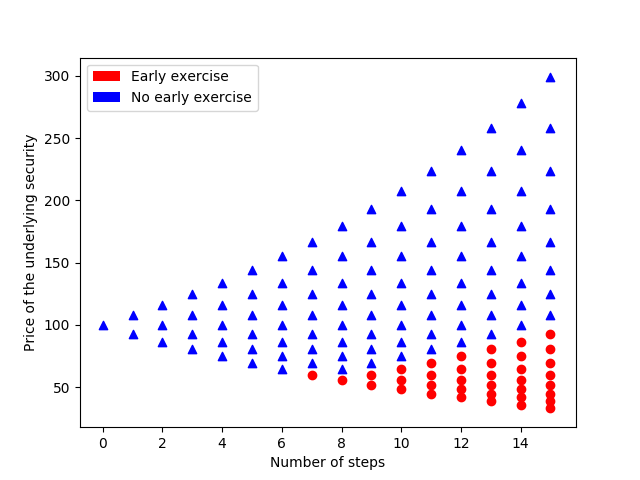
\includegraphics[width=.8\linewidth]{plots/n_15_r_001.png}  
			\caption{Tree with depth 15}
			\label{fig2:sub-second}
		\end{subfigure}
		
		
		\begin{subfigure}{.5\textwidth}
			\centering
			% include third image
			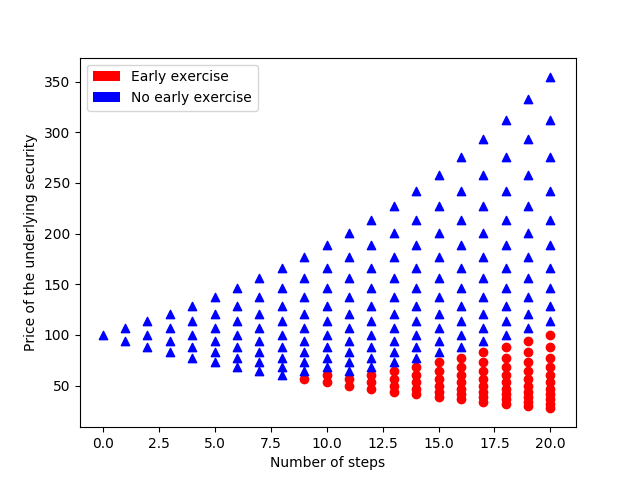
\includegraphics[width=.8\linewidth]{plots/n_20_r_001.png}  
			\caption{Tree with depth 20}
			\label{fig2:sub-third}
		\end{subfigure}
		\begin{subfigure}{.5\textwidth}
			\centering
			% include fourth image
			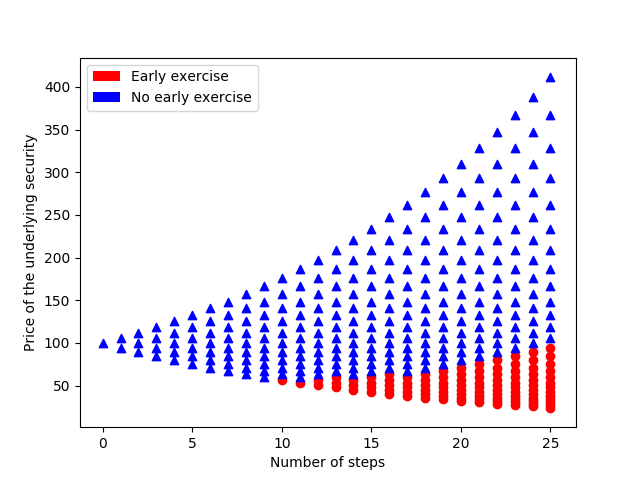
\includegraphics[width=.8\linewidth]{plots/n_25_r_001.png}  
			\caption{Tree with depth 25}
			\label{fig2:sub-fourth}
		\end{subfigure}
		\caption{Depth variation with interest rate 0.1\%}
		\label{fig:fig2}
	\end{figure}
\end{small}

From the figures we can observe that with the variation of the depth of the tree for the same interest rate, the exercise frontier gets delayed. This means that in the depth of the tree is increased the points of early exercise move further down in the tree.

\section*{Other pricing model}
\addcontentsline{toc}{section}{\protect\numberline{Other pricing model}}

We also went ahead and implemented other popular pricing models like the Jarrow-Rudd model, Titan model, Jarrow-Rudd Risk Neutral, and CRR model with drift. 
\linebreak
\linebreak
\subsection*{Jarrow-Rudd model}
\addcontentsline{toc}{subsection}{\protect\numberline{Jarrow-Rudd model}}
The Jarrow-Rudd model($Y_t$) is based on the log-transformation of the binomial model. The figure below shows the exercise frontier for an American option priced using a Jarrow-Rudd model. 

\begin{figure}[H]
	\centering
	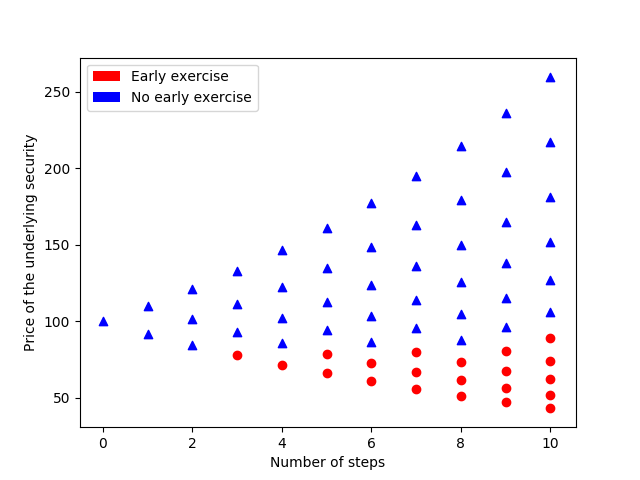
\includegraphics[scale=0.6]{plots/JRmodel.png}
	\caption{Exercise frontier obtained using Jarrow Rudd Model with r=5\%}
\end{figure}

\begin{equation*}
	Y_t = \log(S_t)
\end{equation*}

From Black-Scholes model we can conclude that.
\begin{equation*}
	\begin{aligned}
		Y_t ~ \mathcal{N}(Y_0 + (r-\sigma^2/2)\Delta t,\sigma^2\Delta t)
	\end{aligned}	
\end{equation*}

The probability for the risk neutral measure in the Jarrow-Rudd model is set to $\frac{1}{2}$. Using this probability we get the value of u and d as.

\begin{equation*}
	\begin{aligned}
		u &= e^{(r-\sigma^2/2)\Delta t + \sigma \Delta t} \\
		d &= e^{(r-\sigma^2/2)\Delta t - \sigma \Delta t}
	\end{aligned}
\end{equation*}

\subsection*{Titan model}
\addcontentsline{toc}{subsection}{\protect\numberline{Titan model}}
The Titan model matches the first three moments of the binomial model to the first three moments of a lognormal distribution.

\begin{equation*}
	\begin{aligned}
		&pu + (1-p) = e^{r\Delta t}\\
		&pu^2 + (1-p)d^2 = (e^{r\Delta t})^2 e^{\sigma^2 \Delta t}\\
		&pu^3 + (1-p)d^3= (e^{r\Delta t})^3 (e^{\sigma^2\Delta t})^3
	\end{aligned}
\end{equation*}

These equation can be solved to get the following parameters values.

\begin{equation*}
	\begin{aligned}
	&v = e^{\sigma^2\Delta t}\\
	&u = 0.5 e^{r\Delta t} v(v+1+\sqrt{v^2 +2v -3})\\
	&u = 0.5 e^{r\Delta t} v(v+1-\sqrt{v^2 +2v -3}) \\
	&p = \frac{e^{r\Delta t} -d}{u-d }
	\end{aligned}
\end{equation*}

The implementation for Titan model can be found in the code attached. The figure below shows the exercise frontier for an American option obtained using a Titan model.

\begin{figure}[H]
	\centering
	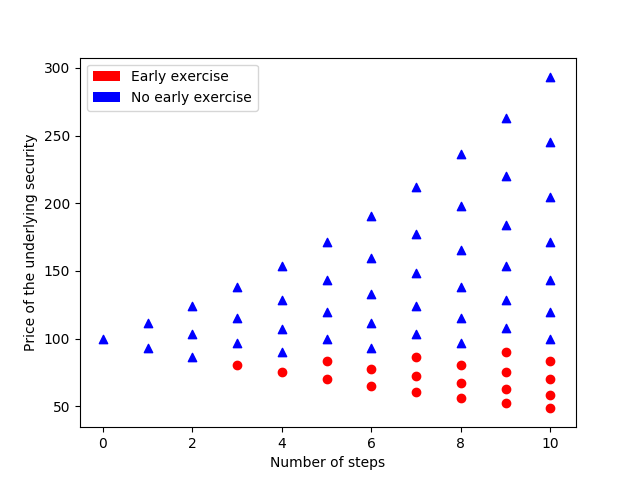
\includegraphics[scale=0.6]{plots/Titanmodel}
	\caption{Exercise frontier obtained using Titan model with r=5\%}
\end{figure}

\subsection*{Jarrow-Rudd risk neutral model}
\addcontentsline{toc}{subsection}{\protect\numberline{Jarrow Rudd Risk neutral measure}}
Jarrow-Rudd risk neutral model is a slight modification on the standard Jarrow-Rudd model. We use the same values for u and d, however instead of $p=\frac{1}{2}$ we use the standard risk neutral definition for $p$.

\begin{equation*}
	\begin{aligned}
	u &= e^{(r-\sigma^2/2)\Delta t + \sigma \Delta t} \\
	d &= e^{(r-\sigma^2/2)\Delta t - \sigma \Delta t} \\
	p &= \frac{e^{r\Delta t} -d }{u-d}
	\end{aligned}
\end{equation*}

The implementation for Jarrow-Rudd risk neutral model can be found in the code attached. The figure below shows the exercise frontier for an American option obtained using a Jarrow-Rudd risk neutral model.

\begin{figure}[H]
	\centering
	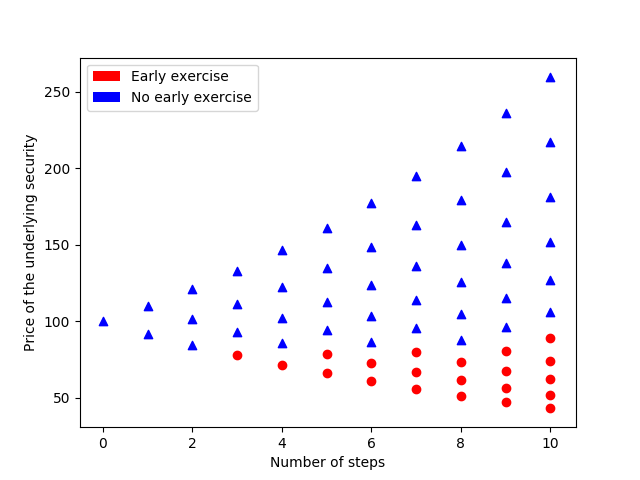
\includegraphics[scale=0.6]{plots/JRRisk}
	\caption{Exercise frontier obtained using Jarrow-Rudd risk neutral model with r=5\%}
\end{figure}


\subsection*{CRR model with drift}
\addcontentsline{toc}{subsection}{\protect\numberline{CRR model with drift}}
The CRR model with drift is a slight modification on the standard CRR model. In this model an arbitrary drift is applied to the parameters of the model and new parameters are given by.

\begin{equation*}
	\begin{aligned}
		&u = e^{\eta\Delta t + \sigma \sqrt{\frac{T}{n}} } \\
		&d = e^{\eta\Delta t -\sigma \sqrt{\frac{T}{n}} } \\
		&p = \frac{e^{r\Delta -d}}{u - d}
	\end{aligned}
\end{equation*}

The drift term is added so that the lattice of security prices can be moved up or down around the current asset price $S_0$ so that more prices can expire in the money. The implementation for CRR model with drift can be found in the code attached. The figure below shows the exercise frontier for an American option obtained using a CRR model with drift.

\begin{figure}[H]
	\centering
	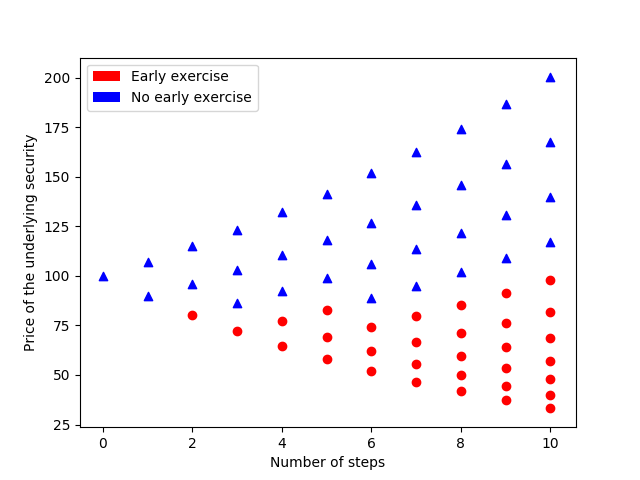
\includegraphics[scale=0.6]{plots/CRRdrift}
	\caption{Exercise frontier obtained using CRR model with $\eta=-0.1$ and $r=0.5\%$}
\end{figure}

\chapter*{Finite difference method for American options}
\addcontentsline{toc}{chapter}{\protect\numberline{Finite difference method for American option}}

\section*{Generating the matrix}
\addcontentsline{toc}{section}{\protect\numberline{Generating the matrix}}
We know that the matrix is A is defined by.

\begin{equation*}
	(AP)_j=\frac{\sigma^2x_j^2}{2}\bigg(\frac{-P^n_{j-1}+2P^n_{j}-P^n_{j+1}}{h^2}\bigg)-rx_j\bigg(\frac{P^n_{j+1}-P^n_{j}}{h}\bigg)+rP^n_{j}
\end{equation*}

$(AP)_j$ is a linear function of the components of the components of P. The code to generate the matrix is shown below.
\\
\begin{python}
	x = np.array([h*j for j in range(M+1)])
	t = np.array([DELTA_T*j for j in range(N)])
	A = [[0 for i in range(M+1)] for j in range(M+1)]
	for i in range(M):
 	 if(i>0):
	  A[i][i-1] = - (((SIGMA**2)*(x[i]**2))/(2*(h**2))) 
	  A[i][i] =  (((SIGMA**2)*(x[i]**2))/((h**2))) + (r*x[i]/h) + r
	  A[i][i+1] = - (((SIGMA**2)*(x[i]**2))/(2*(h**2))) - (r*x[i]/h)
	A = np.array(A)
\end{python}

\section*{Discretization scheme}
\addcontentsline{toc}{section}{\protect\numberline{Discretization Scheme}}

The explicit Euler scheme given to us is as follows. 

\begin{equation*}
\min{\bigg\{\frac{P_j^{n+1}-P_j^{n}}{\Delta t}+\frac{\sigma^2x_j^2}{2}\bigg(\frac{-P^n_{j-1}+2P^n_{j}-P^n_{j+1}}{h^2}\bigg)-rx_j\bigg(\frac{P^n_{j+1}-P^n_{j}}{h}\bigg)+rP^n_{j},\ P_j^{n+1}-g(x_j)\bigg\}}=0
\end{equation*}

\begin{equation*}
P_{M+1}^{n+1}=0
\end{equation*}

Not considering the stopping condition we can see that the explicit scheme is given by. 

\begin{equation*}
	\begin{aligned}
		& \min{\bigg\{\frac{P_j^{n+1}-P_j^{n}}{\Delta t}+\frac{\sigma^2x_j^2}{2}\bigg(\frac{-P^n_{j-1}+2P^n_{j}-P^n_{j+1}}{h^2}\bigg)-rx_j\bigg(\frac{P^n_{j+1}-P^n_{j}}{h}\bigg)+rP^n_{j},\ P_j^{n+1}-g(x_j)\bigg\}}=0 \\
	    &\implies \min{\bigg\{\frac{P_j^{n+1}-P_j^{n}}{\Delta t}+AP^n,P_j^{n+1}-g(x_j)\bigg\}}=0 \\
	    &\implies P_j^{n+1}+\min{\bigg\{-P_j^{n}+\Delta tAP^n,-g(x_j)\bigg\}}=0\\
		&\implies P_j^{n+1} = - \min{\bigg\{-P_j^{n}+\Delta tAP^n,-g(x_j)\bigg\}}\\
		&\implies P_j^{n+1} = \max {\bigg\{P_j^{n}-\Delta tAP^n,g(x_j)\bigg\}}\\
		&\implies P^{n+1} = \max{\bigg\{P^{n} + \Delta t AP^{n},\phi \bigg\}}
	\end{aligned}
\end{equation*}

\section*{Stability of explicit scheme}
\addcontentsline{toc}{section}{\protect\numberline{Stability of explicit scheme}}

The solution to the explicit scheme is unstable and blows up as the value of M is increased.  

\begin{figure}[H]
	\centering
	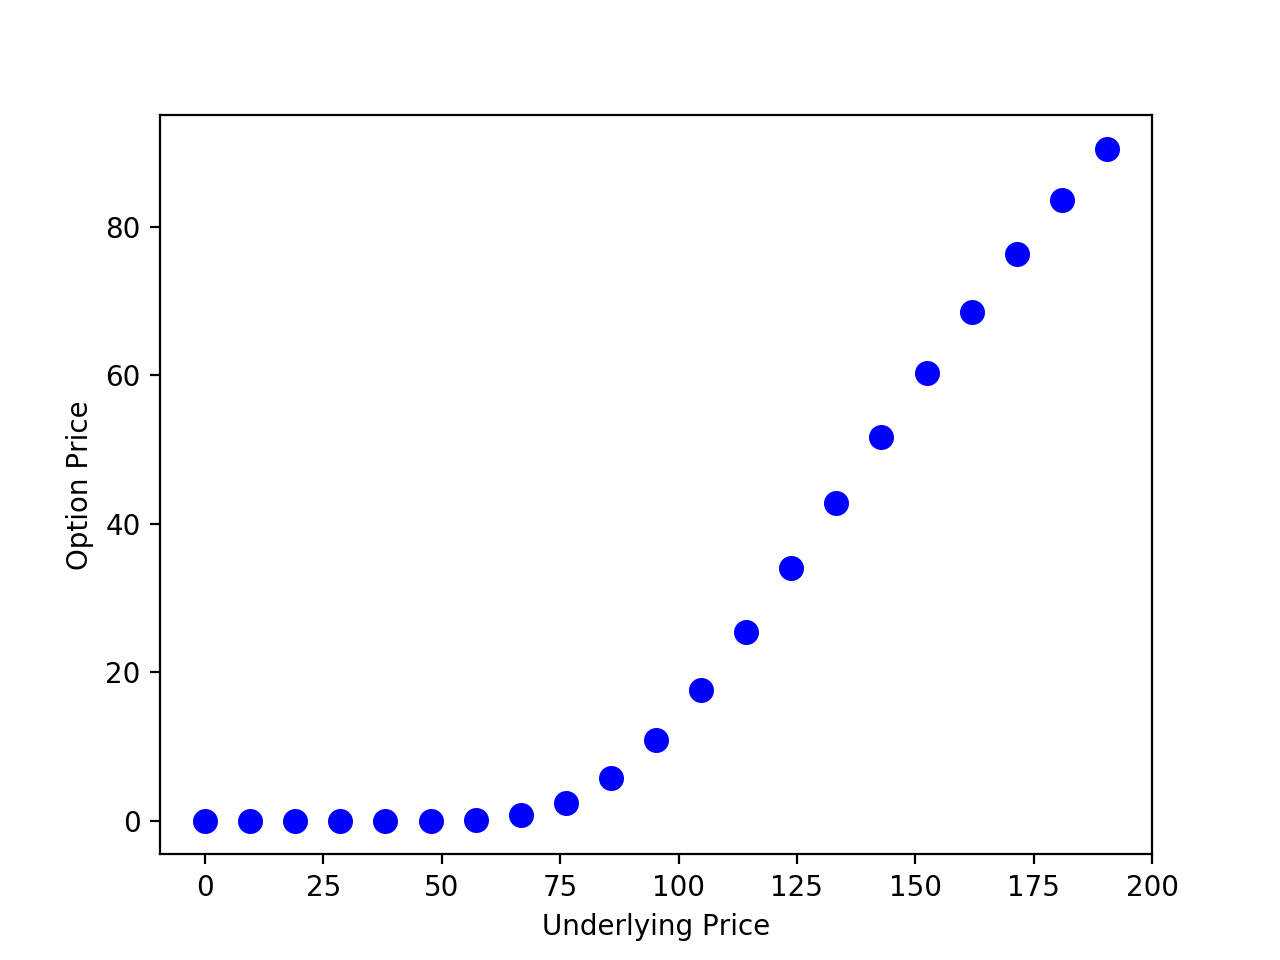
\includegraphics[height=10cm,width=13cm]{Explicit}
	\caption{Explicit Scheme Solution for Different Values of $S$ at $t= 0$}
\end{figure}

The figure shows the solution to the explicit solution scheme for $M=20$. The code used to generate the solution is shown below.

\begin{python}
def phi_call(x):
 payoff = max(x-K,0)
 return payoff

def phi_put(x):
 payoff = max(K-x,0) 
 return payoff

P = np.array([[0.0 for i in range(M+1)] for j in range(N+1)])

for i in range(M+1):
 P[0][i] = phi_call(x[i])


for i in range(1,N+1):
 P[i] = np.maximum(P[i-1]-DELTA_T*np.matmul(A,P[i-1]),np.array([phi_call(x[j]) for j in range(M+1)])) 

print("Explicit Euler Pricing Solution:")
print(P[N])
explicit_sol = P[N]
\end{python}

\section*{Implicit Euler scheme}
\addcontentsline{toc}{section}{\protect\numberline{Implicit Euler Scheme}}

We know that.

\begin{equation*}
	\begin{aligned}
		&\Bigg[\frac{\partial p}{\partial q}\Bigg]_{ij} = \frac{\partial p_i}{\partial q_j}  \hspace{2cm} \text{for any vector $p$ and $q$} \\
		& (Bx-b)_i = \sum_{a=1}^{M+1}(B_{ia}x_a)-b_i\hspace{2cm} \text{ for $i=0,1...M+1$}
	\end{aligned}
\end{equation*}

From the above results we can conclude that. If $(Bx-b)_i \leq (x-\phi)$.

\begin{equation*}
	\begin{aligned}
		& \Bigg[\frac{\partial F(x)}{\partial x} \Bigg]_{ij} = \Bigg[\frac{\partial (Bx-b)}{\partial x} \Bigg]_{ij} \\
		&= \frac{\partial (Bx-b)_i}{\partial x_j} \\
		&= \frac{\partial (\sum_{a=1}^{M+1}(B_{ia}x_a)-b_i)}{\partial x_j}\\
		&=B_{ij}
	\end{aligned}
\end{equation*}

Now considering the case when   $(Bx-b)_i > (x-\phi)$.

\begin{equation*}
	\begin{aligned}
		&\Bigg[\frac{\partial F(x)}{\partial x} \Bigg]_{ij} \\
		&= \bigg[\frac{\partial (x-\phi)}{\partial x}\bigg]_{ij} \\
		&= \frac{\partial (x-\phi)_i}{\partial x_j} \\
		&= \frac{\partial (x_i-\phi_i)}{\partial x_j} \\
		&= \delta_{ij}
	\end{aligned}
\end{equation*}

The above is the required result.

\section*{Newton's method for implicit scheme}

The implementation of Newton-Raphson algorithm for the implicit scheme is shown below.
\linebreak
\begin{python}
B = np.identity(M+1) + DELTA_T*A
P = [np.array([np.random.uniform() for i in range(M+1)]) for i in range(N+1)]
for i in range(M+1):
 P[0][i] = phi_call(x[i])

def F(a,b):
 return np.minimum(np.matmul(B,a)-b,a-P[0])

def deriv(a,b,i,j):
 p = np.matmul(B,a)-b
 q = a - P[0]
 if(p[i]<=q[i]):
  return B[i][j]
 else:
  if(i==j):
   return 1
  else:
   return 0

def F_dash(a,b):
 K = [[0 for i in range(M+1)] for i in range(M+1)]
 for i in range(M+1):
  for j in range(M+1):
   K[i][j] = deriv(a,b,i,j)
 return np.array(K)

for j in range(1,N+1):
 for i in range(num_iterations):
  P[j] = P[j] - np.matmul(np.linalg.pinv(F_dash(P[j],P[j-1])),F(P[j],P[j-1]))

\end{python}

We run the code for 1000 iterations and find that solution remains stable. Shown below are the results for the option price for M=20 and M=50.

\begin{figure}[H]
	\centering
	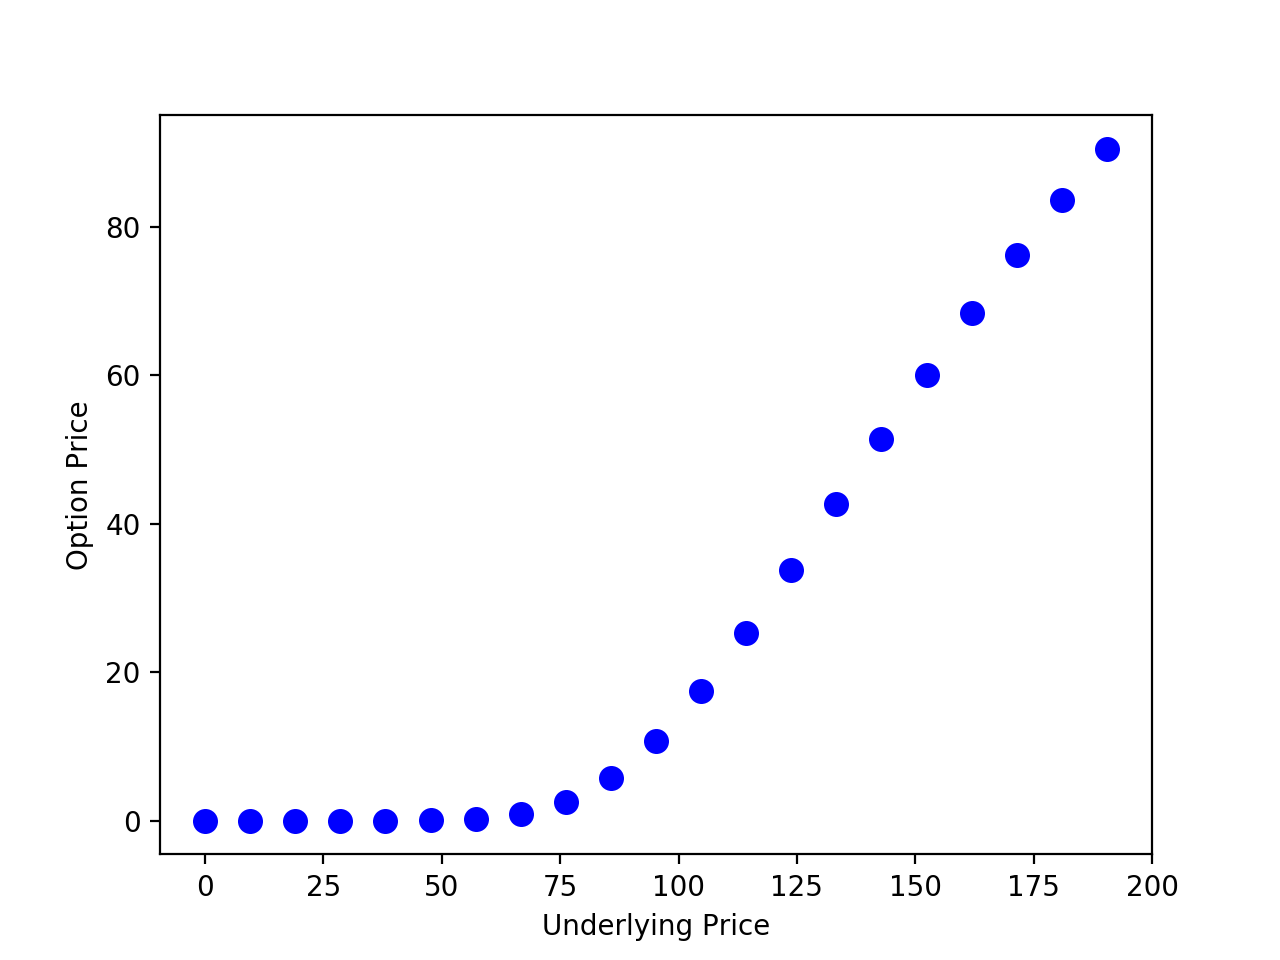
\includegraphics[height=10cm,width=13cm]{Implicit_20}
	\caption{Implicit Scheme Solution for Different Values of $S$ at $t= 0$ and $M= 20$}
\end{figure}

\begin{figure}[H]
	\centering
	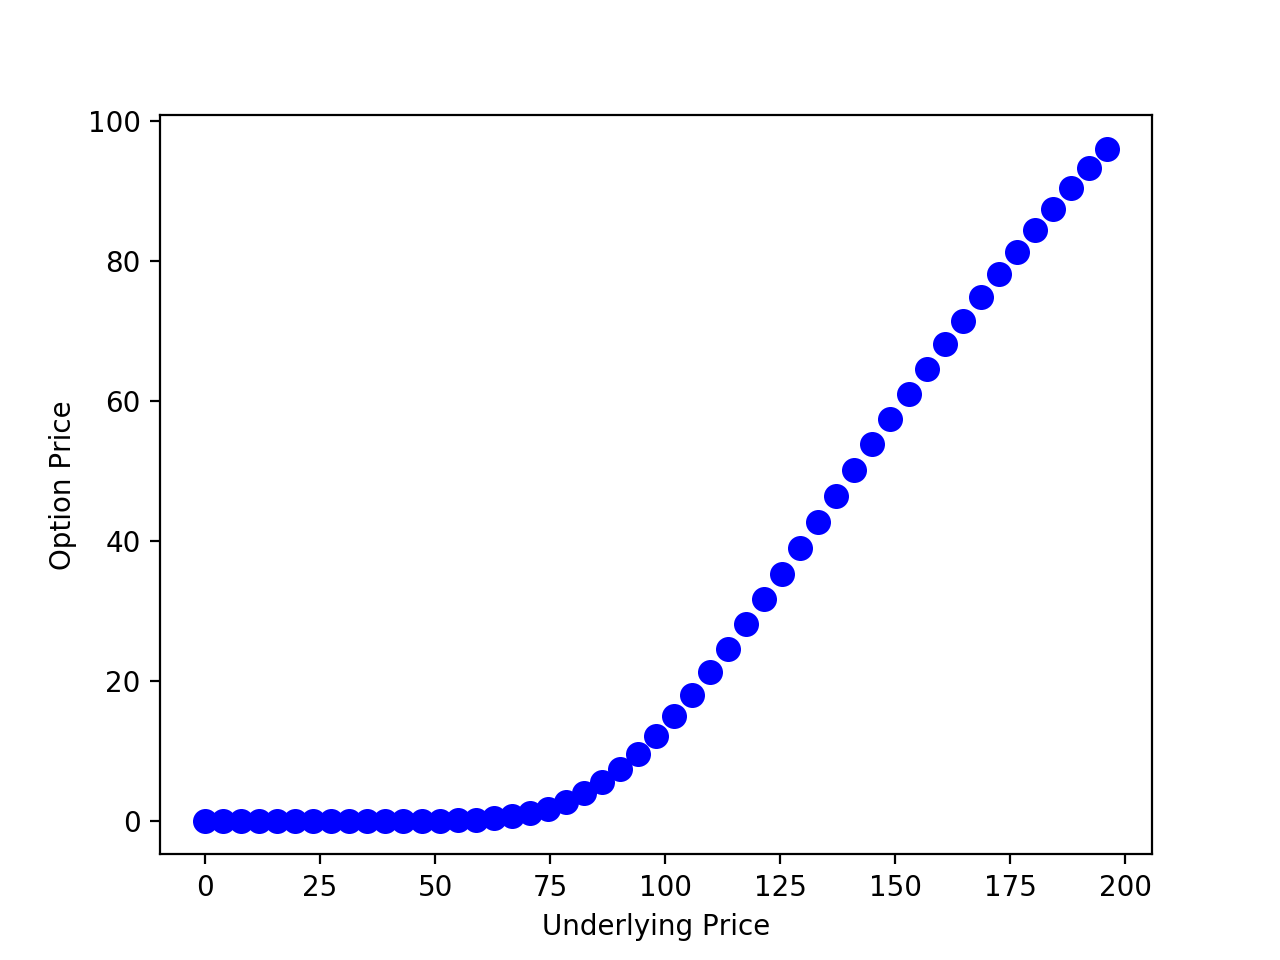
\includegraphics[height=10cm,width=13cm]{Implicit_50}
	\caption{Implicit Scheme Solution for Different Values of $S$ at $t= 0$ and $M= 50$}
\end{figure}

\end{document}